%%%%%%%%%%%%%%%%%%%%%%%%%%%%%%%%%%%%%%%%%
% University/School Laboratory Report
% LaTeX Template
% Version 3.1 (25/3/14)
%
% This template has been downloaded from:
% http://www.LaTeXTemplates.com
%
% Original author:
% Linux and Unix Users Group at Virginia Tech Wiki 
% (https://vtluug.org/wiki/Example_LaTeX_chem_lab_report)
%
% License:
% CC BY-NC-SA 3.0 (http://creativecommons.org/licenses/by-nc-sa/3.0/)
%
%%%%%%%%%%%%%%%%%%%%%%%%%%%%%%%%%%%%%%%%%

%----------------------------------------------------------------------------------------
%	PACKAGES AND DOCUMENT CONFIGURATIONS
%----------------------------------------------------------------------------------------

\documentclass{article}

\usepackage[version=3]{mhchem} % Package for chemical equation typesetting
\usepackage{siunitx} % Provides the \SI{}{} and \si{} command for typesetting SI units
\usepackage{graphicx} % Required for the inclusion of images
\usepackage{natbib} % Required to change bibliography style to APA
\usepackage{amsmath} % Required for some math elements 
\usepackage[export]{adjustbox} % loads also graphicx
\usepackage{listings}
\usepackage{matlab-prettifier}
\usepackage{float}


\usepackage{caption}
\usepackage{subcaption}


\usepackage{xcolor}

\DeclareCaptionFont{white}{\color{white}}
\DeclareCaptionFormat{listing}{%
  \parbox{\textwidth}{\colorbox{gray}{\parbox{\textwidth}{#1#2#3}}\vskip-4pt}}
\captionsetup[lstlisting]{format=listing,labelfont=white,textfont=white}
\lstset{frame=lrb,xleftmargin=\fboxsep,xrightmargin=-\fboxsep}


\setlength\parindent{0pt} % Removes all indentation from paragraphs

\renewcommand{\labelenumi}{\alph{enumi}.} % Make numbering in the enumerate environment by letter rather than number (e.g. section 6)

%\usepackage{times} % Uncomment to use the Times New Roman font

%----------------------------------------------------------------------------------------
%	DOCUMENT INFORMATION
%----------------------------------------------------------------------------------------

\title{Two-Dimensional Ising Model \\ of Ferromagnetic Micro-lattice} % Title

\author{Trent \textsc{Yarosevich}} % Author name

\date{\today} % Date for the report

\begin{document}
\maketitle % Insert the title, author and date
\setlength\parindent{1cm}

\begin{center}
\begin{tabular}{l r}
Date Performed: December 1, 2017 \\ % Date the experiment was performed
Instructor: & Professor Lionel Mathelin % Instructor/supervisor
\end{tabular}
\end{center}

% If you wish to include an abstract, uncomment the lines below
% \begin{abstract}
% Abstract text
% \end{abstract}

%----------------------------------------------------------------------------------------
%	SECTION 1
%----------------------------------------------------------------------------------------

\section{Objective}

To analyze a simulation of a simplified 2D Ising model of ferromagnetic material and examine its behavior as its magnetization fluctuates at a non-zero temperature. This model is subjected to a magnetic field $H = H e_z$ at temperature $T$.

% If you have more than one objective, uncomment the below:
%\begin{description}
%\item[First Objective] \hfill \\
%Objective 1 text
%\item[Second Objective] \hfill \\
%Objective 2 text
%\end{description}


\noindent The structure of the simulation is a lattice $S$ modeled in Matlab as a matrix of $NxN$ size, with sites of index i (row) and j (column) indicating magnetic moment.
\begin{equation}
S_{ij} = \pm 1, \forall_i, j,
\end{equation}
The magnetization for any given configuration is defined as the sum of all elements
\begin{equation}
M(S) = \sum_{ij} S_{ij}
\end{equation}
and the internal energy of any state $S$ is defined by
\begin{equation}
U(S) = -J\sum_{ij} S_{ij}(S_{i+1, j} + S_{i-1, j} + S_{i,j+1} + S_{i,j-1}) - H\sum_{ij} S_{ij},
\end{equation}
with an intensity of interaction $J > 0.$ When neighboring spins are aligned in the direction of $\textbf{H}$, the internal energy will be minimal, represented in equation 3 by subtracting $H\sum_{ij}S_{ij}.$ \newline


\noindent The substance of the simulation will rely on modeling the effect of non-zero temperatures on the system, which result in fluctuations that cause the spins at each simulated site to configure at random. The probability of distribution for any given state $S$ is defined by 
\begin{equation}
P_S(S) = \frac{exp(-\beta U(S))}{Z},
\end{equation}
with $Z$ given by the Boltzmann partition function
\begin{equation}
Z := \sum_{{S}} exp(-\beta U(S)).
\end{equation} 
This in turn allows for the calculation of the mean magnetization of all possible configurations for some given values $J, H$ and $\beta.$ In practice, however, this is not a tenable approach in practice, however, as calculating $Z$ for all possible $2^{N^2}$ matrices $S$ is a computational obstacle, even for trivially sized matrices. Instead, this simulation will make use of the Markov-chain Monte-Carlo method and the Metropolis-Hasting algorithm.
%----------------------------------------------------------------------------------------
%	SECTION 2
%----------------------------------------------------------------------------------------

\section{Outline of Markov-Chain Approach}

The Metropolis algorithm will be implemented in the following steps. \\

\noindent
\textbf{1.)} A random matrix of size $NxN$ will be initialized with randomly assigned values of either -1 or 1, and will be the first state $S^{(1)}$ whose mean magnetization will be denoted $M(S).$ The following Matlab code is used to accomplish this:


\begin{lstlisting}[style=Matlab-editor, label=some-code,caption= ]
% Initialize Matrix size.
N = 50;
% Initialize an NxN matrix of ones and subtract an NxN matrix with randomly
% assigned entries of -2.
S =ones(N,N) - 2 * randi([0 1], N, N); 
\end{lstlisting}
\paragraph{} \hspace{0pt} \\
\noindent
\textbf{2.)} A potential new new state $S$ is created in accordance with the Ising model by changing the state of the spin at a randomly chosen site to an opposite value:
\begin{equation}
S^{Prop}_{ij} = -S^{(k)}_{ij}.
\end{equation}
The probability $r$ of acceptance of this new state is then evaluated:
\begin{equation}
r = min(1,\frac{P(S^{Prop})}{P(S^{k})})
\end{equation}
which simplifies to the following, since it merely depends on $\Delta U:$
\begin{equation}
r = min(1, exp(-\beta \Delta U)).
\end{equation}
$\Delta U$ in turn is defined by $U(S^{prop}) - U(S^{(k)})$ with $U(S)$ given by equation (3). Recall per equation (6) that the only difference between $S^{prop}$ and $S^{(k)}$ is the opposite value at location $S_{ij}$. Thus when we take the sum of all sites to calculate the mean magnetization (equation (2)) all values in $\sum_{ij}S^{(k)}_{ij}$ and $\sum_{ij}S^{Prop}_{ij}$ are identical, with the exception of $S_{ij}$ and its surrounding 4 sites. As a result, all the identical values cancel, and $\Delta U$ can be calculated substituting $-S_{ij}^{(k)}$ in place of $S_{ij}^{Prop}$. The result are the following contributions to $\Delta U$ at some site $S_{ij}:$
\begin{equation}
\begin{aligned}
-J (-S_{ij})(S_{i+1, j} + S_{i-1, j} + S_{i,j+1} + S_{i,j-1})- H(-S_{ij}) \\ - ( -JS_{ij}(S_{i+1, j} + S_{i-1, j} + S_{i,j+1} + S_{i,j-1}) - HS_{ij})
\end{aligned}
\end{equation}
simplifying to 
\begin{equation}
2JS_{ij}(S_{i+1, j} + S_{i-1, j} + S_{i,j+1} + S_{i,j-1}) + 2HS_{ij}.
\end{equation}
Each adjacent site contributes to $\Delta U$ in relation to one site $S_{ij}$ only, thus all four contribute
\begin{equation}
2JS_{ij}(S_{i+1, j} + S_{i-1, j} + S_{i,j+1} + S_{i,j-1})
\end{equation}
and in turn $\Delta U$ simplifies to:


\begin{equation}
4J (S^{(k)}_{ij})(S^{(k)}_{i+1, j} + S^{(k)}_{i-1, j} + S^{(k)}_{i,j+1} + S^{(k)}_{i,j-1}) + 2HS^{(k)}_{ij}.
\end{equation}

\noindent
\textbf{3.)} If $\Delta U < 0$, the acceptance probability $r =1$ and $S^{Prop}$ becomes $S^{(k+1)}.$ If $\Delta U > 0$, the candidate state can still be accepted depending on thermal fluctuations. This is evaluated by comparing $r$ to some probability $t$ drawn from the family of real-valued variables with uniform distribution across [0, 1]. If $r > t$ the state is accepted, and if not the site remains unchanged and $S^{(k+1)} = S^{(k)}$.
\paragraph{} \hspace{0pt} \\
\noindent
\textbf{4.)} The magnetization for the new state $M(S^{(k+1)}$ is then calculated and the algorithm progresses to the next iteration.

%----------------------------------------------------------------------------------------
%	SECTION 3
%----------------------------------------------------------------------------------------

\section{Initial Motivation and Simulation Details}

Before proceeding to the full simulation with a dynamic field $\textbf{H}$, we will consider a limited example of the Metropolis Algorithm for illustrative purposes. In this case, the strength of interaction $J$ will be taken as 1, the field strength 
Before proceeding to the full simulation with a dynamic field $\textbf{H}$ as .1, and $\beta$ as .5. We will consider a micro-lattice of 50x50 sites over $N_r = 10^5$ realizations. The following are plots of the initial state $S^{(1)}$ and final state $S^{(N_r)}$: 
\begin{figure}[H]
  \centering
  \begin{minipage}[b]{0.49\textwidth}
    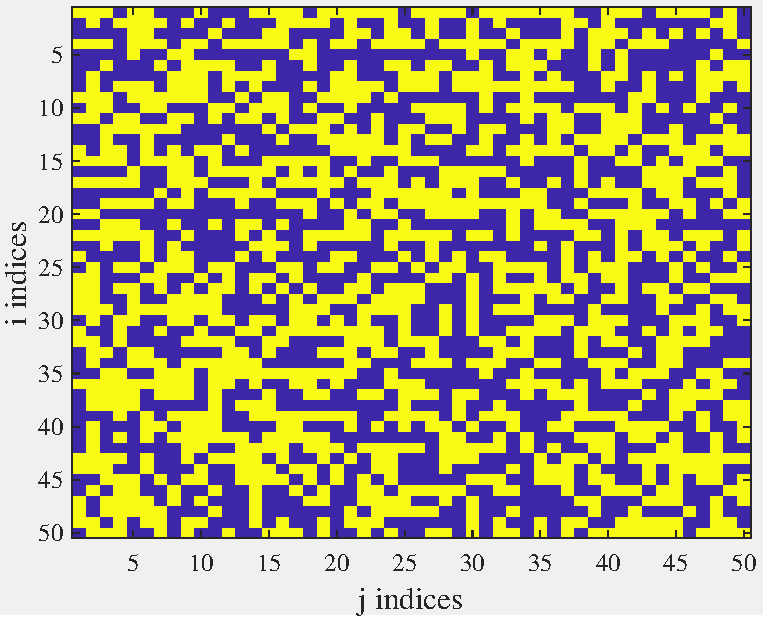
\includegraphics[width=\textwidth]{initialS.pdf}
    \caption{$N_1$ Realization}

  \end{minipage}
  \hfill
  \begin{minipage}[b]{0.49\textwidth}
    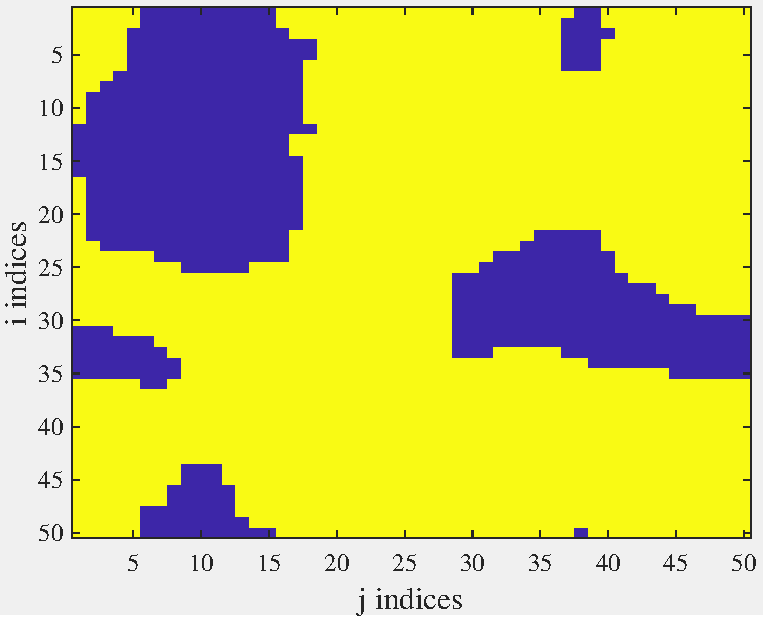
\includegraphics[width=\textwidth]{finalS.pdf}
    \caption{$N_r$ Realizations}

  \end{minipage}
\end{figure}

\noindent Furthermore, when the magnetization $M$ is plotted over $N_r$ realizations in the presence of a stronger field $\textbf{H} = .5$ we see that it stabilizes at a uniform spin of 1.
\\
\begin{figure}[H]
  \centering
  \begin{minipage}[b]{0.49\textwidth}
    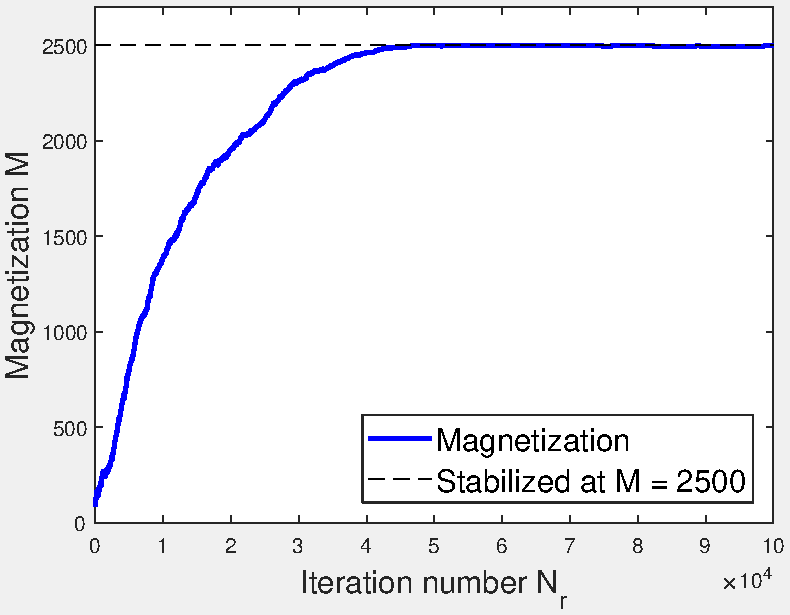
\includegraphics[width=\textwidth]{Mplot.pdf}
    \caption{Magnetization $M$ over time}

  \end{minipage}
  \hfill
  \begin{minipage}[b]{0.49\textwidth}
    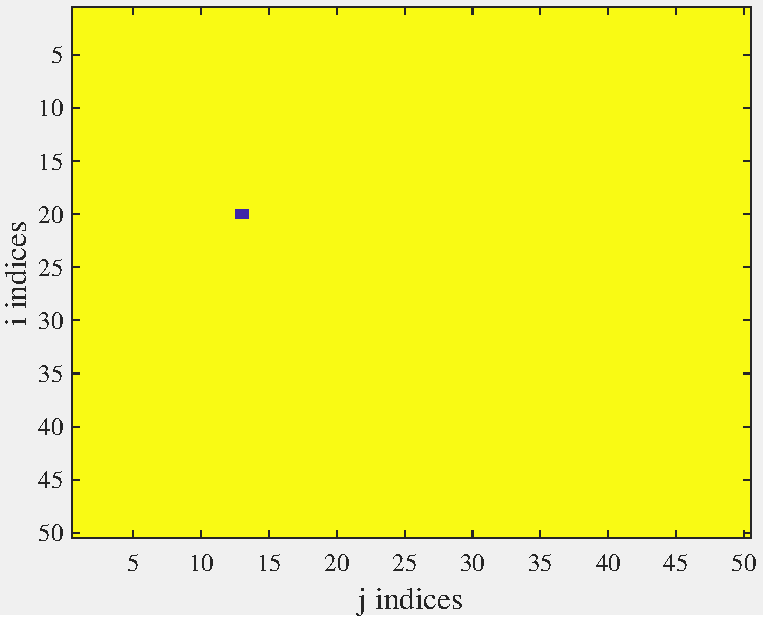
\includegraphics[width=\textwidth]{Suniform.pdf}
    \caption{Stabilized state $S_r$}

  \end{minipage}
\end{figure}

\noindent This tendency toward a uniform spin is to be expected, as Markov chains tend toward a stabilized state. For this reason, the method for calculating mean magnetization used here
\begin{equation}
\overline{M} = N_r^{-1} \sum_{k=1}^{N_r} M(S^{(k)})
\end{equation}
is not well suited to this method, since any such calculated mean would not convey useful information if the simulation spends most of its iterations in a uniform state.
%----------------------------------------------------------------------------------------
%	SECTION 4
%----------------------------------------------------------------------------------------

\section{Simulation with Dynamic $\textbf{H}$ Values}

\noindent The main simulation takes a single initial state of randomly assigned spins $S_1$ and then proceeds simulates the application of a dynamic magnetic field $\textbf{H}$ ranging from -5 to 5 and then back to -5 with 100 total discrete steps. At each value of $\textbf{H}$ the model will proceed through $N_r$ realizations. Note that the state $S_r$ for each value $\textbf{H}$ is retained and becomes $S_1$ for the next $\textbf{H}$ value. The following graph shows how $\overline{M}$ develops over time.
\begin{figure}[H]
\centering
    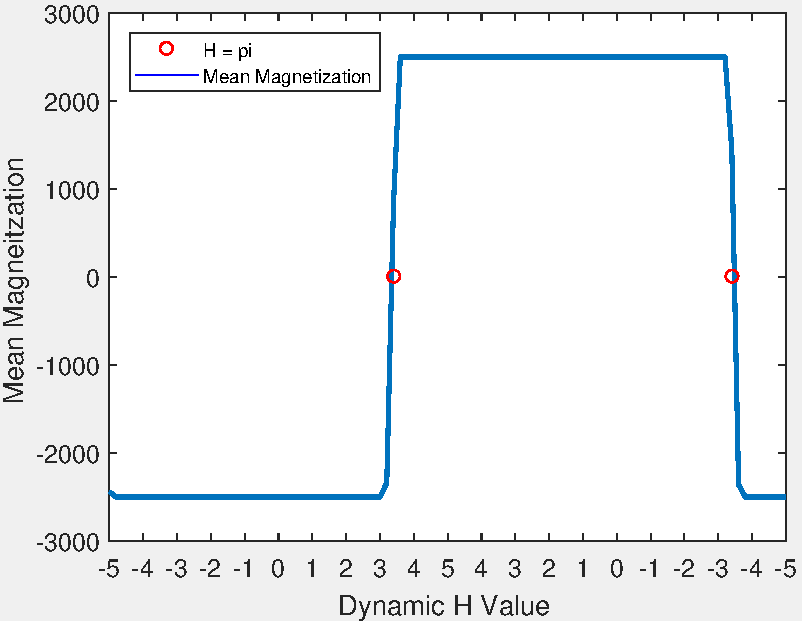
\includegraphics[width=\textwidth]{dynamicHtime.pdf}
	\caption{$\overline{M}$ in with $\textbf{H}$ from -5, 5, -5}
\end{figure}

\noindent In this particular simulation it is clear that when $\textbf{H}$ reaches pi, the effect of the magnetic field is sufficient to flip the spin distribution, and then again after a further $\Delta{H} =10.$ The symmetry of this phenomenon is perhaps more clearly shown with a simple plot with the x-axis defined linearly by the value $\textbf{H}$:
\begin{figure}[H]
\centering
    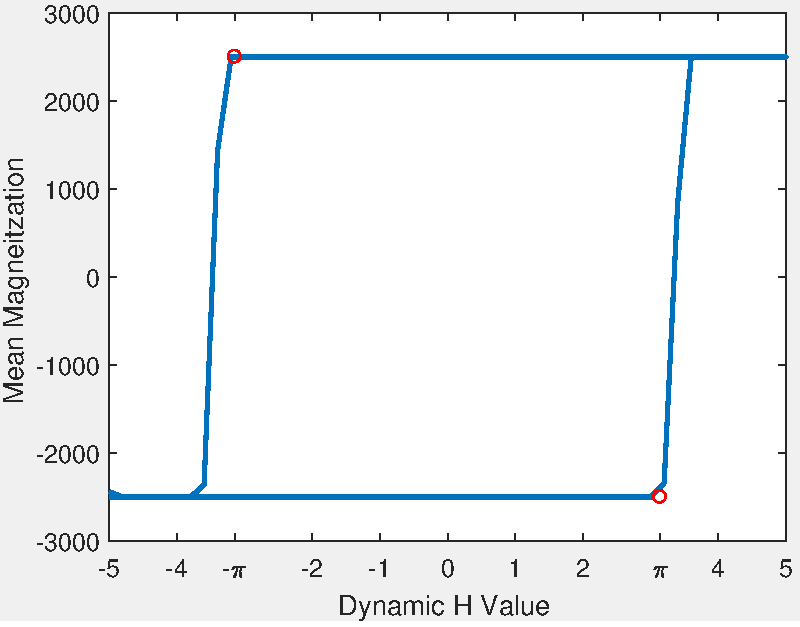
\includegraphics[width=\textwidth]{singleplot.pdf}
	\caption{$\overline{M}$ against linear $\textbf{H}$}
\end{figure}

\section{Conclusions}
On the surface it seems clear that, in the case of the simulation, when $\textbf{H}$ reaches a value of $\pi$ whilst $S$ is stable at $\overline{M} = -N^2$, or when it reaches a value of $-\pi$ while $S$ is stable at $\overline{M} = N^2$, a rapid change in $\overline{M}$ occurs. From this, we could deduce that while $\overline{M}$ is stable and $\textbf{H}$ is greater or less than $\pi$ (depending on the sign of $S$'s uniform spin) that $r$ remains very small and therefore very few changes to $S$ can propagate. 

More contextually, it seems possible that these moments at which $\overline{M}$ rapidly changes corresponds to the rotation of a magnetic field relative to the ferromagnetic lattice. I would hypothesize that as this field rotates, it eventually causes the stable spin to quickly change as the tendencies of the thermal fluctuations change bias. Confirming or disproving this theory in the context of this simulation would require further investigation of how the contributions to $\Delta U$ develop in relation to one another, and how $r$ correspondingly changes over time.


%%----------------------------------------------------------------------------------------
%%	BIBLIOGRAPHY
%%----------------------------------------------------------------------------------------
%
%\bibliographystyle{apalike}
%
%\bibliography{sample}
%
%%----------------------------------------------------------------------------------------


\end{document}
